\documentclass{standalone}
%\usepackage{tkz-fct}
%\usepackage{tkz-euclide}
\usepackage{pgfplotstable}
\usepackage{color}
\usepackage{pgfplots}
\renewcommand*\familydefault{\sfdefault}
\usepackage{sansmath}
\sansmath
\definecolor{gray75}{gray}{0.75}
\begin{document}
\pgfplotsset{every axis x label/.style={at={(current axis.right of origin)},anchor=east}}
\pgfplotsset{every axis y label/.style={at={(current axis.above origin)},anchor=east}}
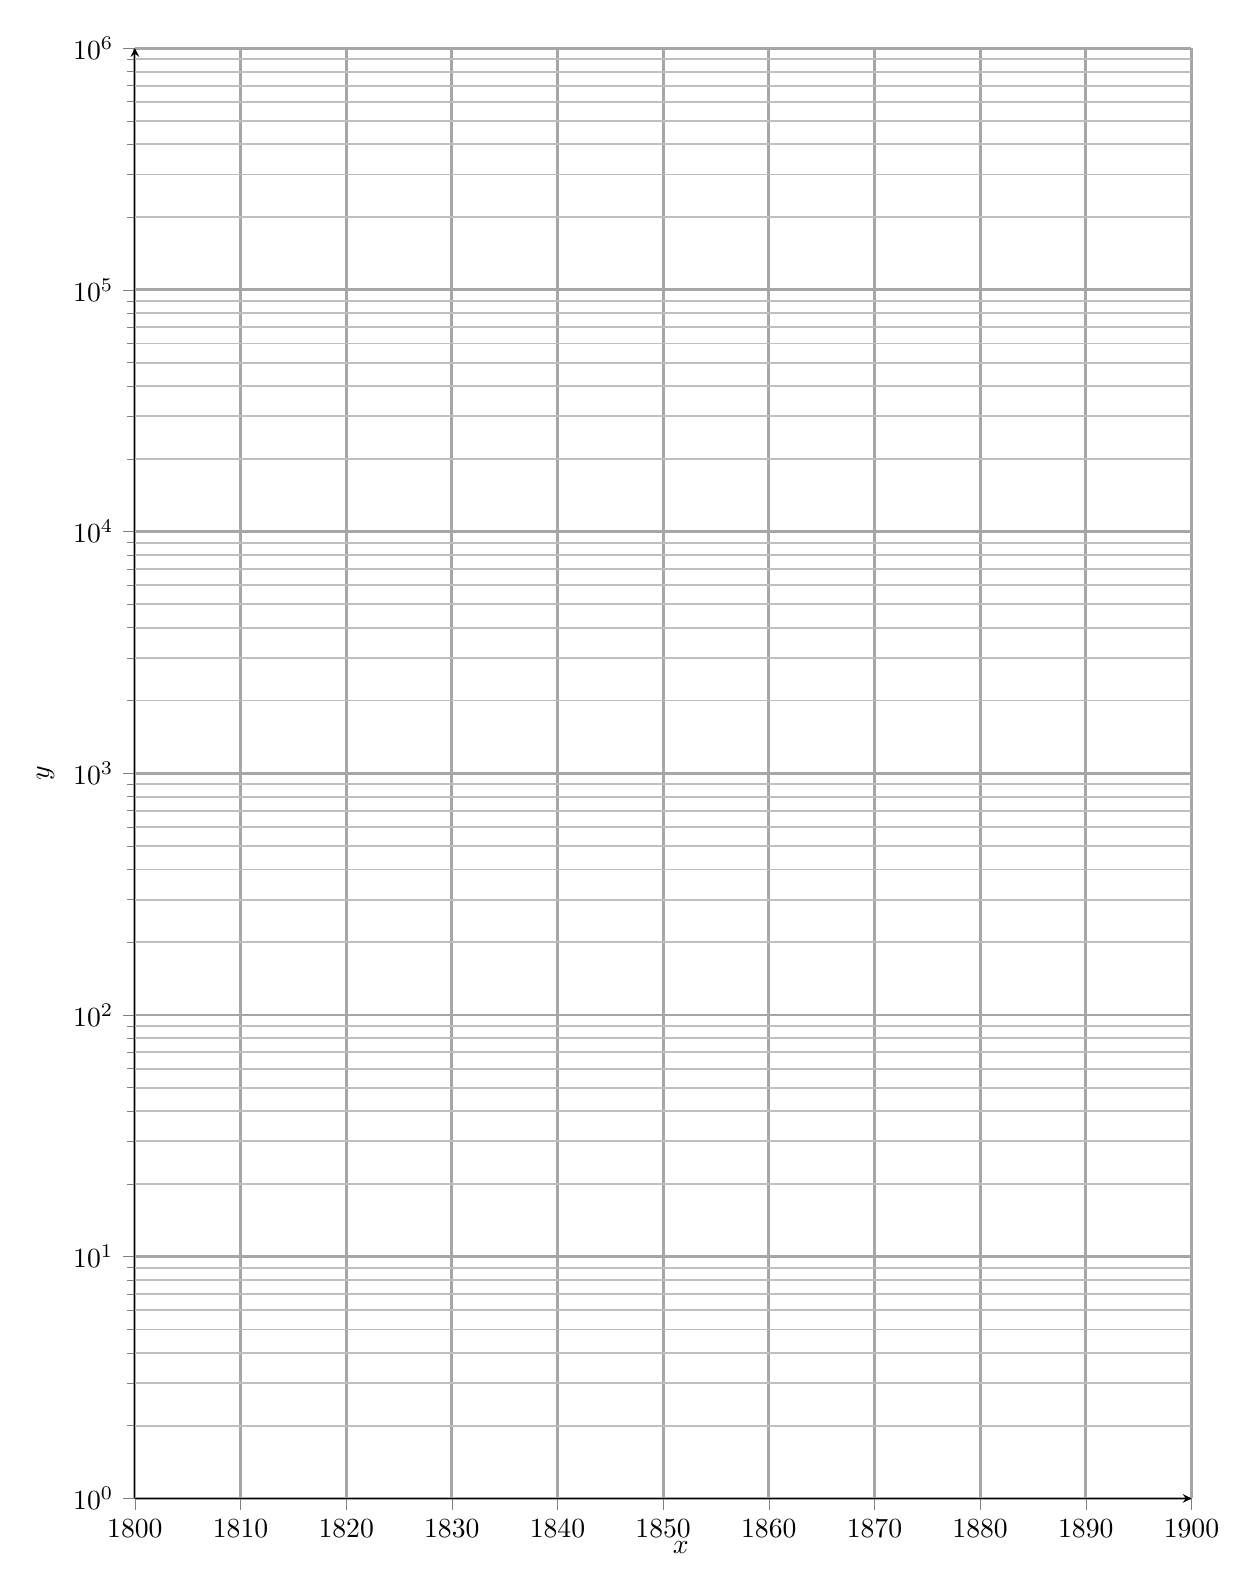
\begin{tikzpicture}
  \begin{axis}[
    /pgf/number format/1000 sep={},
    width=15cm,
    height=20cm,
    grid style={line width=.7pt, draw=gray!50},
    major grid style={line width=1pt,gray!70},
    axis y line={left},
    axis x line={bottom},
    tick align=outside,
    grid=both,
    xlabel = {$x$},
    ylabel = {$y$},
    ymode = log,
    xmin=1800, ymin=1e0, xmax=1900, ymax=1e6,
    x label style={right},
    y label style={above}]
\end{axis}
\end{tikzpicture}
\end{document}
